\section{Câu hỏi 3: Dự báo 7 ngày và so sánh mô hình}
\label{sec:q3}

\subsection{Bài toán và chiến lược dự báo}

Tại mỗi gốc $t$, mô hình phải đưa ra bảy dự báo $\hat{q}_{t+1},\ldots,\hat{q}_{t+7}$.
Báo cáo sử dụng chiến lược \emph{dự báo trực tiếp} \cite{tashman2000}: huấn luyện
riêng một mô hình cho mỗi horizon $h$, thay vì dùng một mô hình đệ quy để dự báo từng bước rồi lấy dự báo
trước làm đầu vào cho bước sau. Cách làm trực tiếp tránh tích lũy sai số qua các
bước và cho phép mỗi horizon học một quan hệ riêng. Đổi lại, cần bảy mô hình và
nhiều tham số hơn.

Ba mô hình được so sánh:

\begin{enumerate}[leftmargin=1.6em]
  \item \textbf{Naive persistence:} $\hat{q}_{t+h}=q_t$ cho mọi $h$. Đây là baseline
  bắt buộc trong dự báo chuỗi có tính dai dẳng cao.
  \item \textbf{Seasonal Naive 365:} $\hat{q}_{t+h}=q_{t+h-365}$, tức lấy giá trị
  cùng ngày của năm trước. Mô hình này kiểm tra giả thuyết chuỗi có mùa vụ năm ổn
  định.
  \item \textbf{LightGBM direct 7:} bảy mô hình cây tăng cường gradient
  \cite{friedman2001,ke2017}, mỗi mô hình dự báo trực tiếp một horizon từ các đặc
  trưng lag, rolling window và lịch.
\end{enumerate}

Cả ba mô hình đều được đánh giá trên cùng 724 gốc Test và cùng 5.068 cặp
$(t,h)$. Việc dùng cùng gốc và cùng horizon bảo đảm so sánh công bằng. Các mô hình
không được phép dùng giá trị tương lai; Seasonal Naive chỉ dùng giá trị cách đó đúng
365 ngày, còn LightGBM chỉ dùng các đặc trưng được tạo từ dữ liệu đến ngày $t$ và
các đặc trưng lịch của ngày mục tiêu.

\subsection{Đặc trưng và mục tiêu delta}

Với mỗi gốc, LightGBM nhận 29 đặc trưng cơ bản: giá trị hiện tại $q_t$; các lag 1,
2, 3, 7, 14, 21, 28 và 30 ngày; trung bình, độ lệch chuẩn, min, max của cửa sổ 7,
14 và 30 ngày; sai phân 1 ngày và 7 ngày; cùng các đặc trưng lịch của ngày gốc
(tháng, ngày trong năm, sin/cos). Ngoài ra, mỗi horizon có thêm sáu đặc trưng lịch
của \emph{ngày mục tiêu}: tháng, ngày trong năm và các biến sin/cos tương ứng. Các
đặc trưng này biết trước nên không gây rò rỉ dữ liệu.

Mục tiêu huấn luyện không phải giá trị tuyệt đối $q_{t+h}$ mà là mức thay đổi
$\Delta_{t,h}=q_{t+h}-q_t$. Mô hình dự báo $\hat{\Delta}_{t,h}$, sau đó cộng lại
$q_t$ để được mức dự báo. Cách làm này được gọi là \emph{delta target} và có tác
dụng “giữ” tính persistence trong mô hình: nếu mô hình học được $\Delta \approx 0$,
nó quay về Naive; nếu học được phần thay đổi, nó cải thiện so với Naive. Đây là lựa
chọn phù hợp với chuỗi có ACF cao, vì mô hình không phải học lại toàn bộ mức lưu
lượng từ đầu.

Cần nhấn mạnh rằng delta target không bảo đảm LightGBM tốt hơn Naive. Nó chỉ giúp
mô hình có một điểm khởi đầu hợp lý. Nếu phần thay đổi chủ yếu là nhiễu, mô hình có
thể học nhiễu và làm sai lệch nhẹ so với Naive. Kết quả thực nghiệm cho thấy đúng
như vậy: LightGBM gần như trùng Naive ở các horizon ngắn và kém hơn một chút ở các
horizon dài.

\subsection{Chọn tham số bằng Validation}

LightGBM được chọn tham số bằng 8 lần thử ngẫu nhiên trên Validation 2020--2021,
với seed 42. Không gian tìm kiếm gồm learning rate $\{0{,}03;0{,}05\}$, số lá
$\{7;15;31\}$, độ sâu $\{3;5;-1\}$, min child samples $\{20;40;80\}$ và
$\lambda \in \{0;1;5\}$. Mỗi lần thử huấn luyện bảy mô hình, dùng early stopping 50
vòng và tối đa 1.000 vòng. Tiêu chí chọn là mean RMSE trên bảy horizon.

\begin{table}[H]
\centering
\footnotesize
\setlength{\tabcolsep}{3.2pt}
\begin{tabular}{rrrrrrrrr}
\toprule
Trial & LR & Leaves & Depth & Min child & Lambda & mean RMSE & mean MAE & mean NSE \\
\midrule
1 & 0{,}03 & 7 & -1 & 40 & 0{,}0 & 5{,}58 & 4{,}45 & 0{,}987 \\
2 & 0{,}03 & 7 & -1 & 20 & 5{,}0 & 5{,}58 & 4{,}45 & 0{,}987 \\
3 & 0{,}03 & 31 & 5 & 20 & 0{,}0 & 5{,}58 & 4{,}45 & 0{,}987 \\
4 & 0{,}03 & 7 & 3 & 80 & 5{,}0 & 5{,}58 & 4{,}45 & 0{,}987 \\
5 & 0{,}03 & 8 & 3 & 80 & 5{,}0 & 5{,}58 & 4{,}45 & 0{,}987 \\
6 & 0{,}05 & 7 & 5 & 80 & 1{,}0 & 5{,}58 & 4{,}45 & 0{,}987 \\
7 & 0{,}03 & 7 & -1 & 40 & 1{,}0 & 5{,}58 & 4{,}45 & 0{,}987 \\
\textbf{8} & 0{,}05 & 7 & 3 & 40 & 0{,}0 & 5{,}57 & 4{,}44 & 0{,}987 \\
\bottomrule
\end{tabular}

\caption{Kết quả 8 lần thử tham số LightGBM trên Validation.}
\label{tab:lgbm-trials}
\end{table}

Bảng~\ref{tab:lgbm-trials} cho thấy các lần thử có kết quả gần như giống nhau:
mean RMSE từ 5,57 đến 5,58 m\textsuperscript{3}/s. Trial 8 được chọn với
learning rate 0,05, 7 lá, độ sâu 3, min child 40 và $\lambda=0$; mean RMSE là 5,57,
mean MAE là 4,44 và mean NSE là 0,987. Khoảng cách giữa trial tốt nhất và trial đầu
tiên chỉ khoảng 0,01 m\textsuperscript{3}/s, nhỏ hơn nhiều so với độ bất định giữa
các năm. Vì vậy không nên diễn giải việc “tối ưu tham số” là nguyên nhân chính tạo
ra kết quả; yếu tố quyết định là cấu trúc đặc trưng và tính dai dẳng của chuỗi.

\subsection{Kết quả Validation}

Bảng~\ref{tab:validation-metrics} so sánh ba mô hình trên Validation. Naive có mean
RMSE 5,54; LightGBM 5,57; Seasonal Naive 65,57. LightGBM thấp hơn Naive về mean NSE
một chút (0,987 so với 0,988). Kết quả này đã dự báo trước kết quả Test: mô hình học
máy không vượt được baseline persistence trên dữ liệu ngoài mẫu.

\begin{table}[H]
\centering
\small
\resizebox{\linewidth}{!}{\begin{tabular}{lrrrrr}
\toprule
Mô hình & mean RMSE & mean MAE & mean NSE & pooled RMSE & pooled NSE \\
\midrule
Naive persistence & 5{,}54 & 4{,}42 & 0{,}988 & 5{,}76 & 0{,}988 \\
Seasonal Naive 365 & 65{,}57 & 59{,}95 & -0{,}612 & 65{,}57 & -0{,}612 \\
LightGBM direct 7 (delta) & 5{,}57 & 4{,}44 & 0{,}987 & -- & -- \\
\bottomrule
\end{tabular}
}
\caption{Chỉ số trên Validation 2020--2021. LightGBM không có pooled validation
trong bảng vì bước chọn tham số chỉ lưu chỉ số theo horizon.}
\label{tab:validation-metrics}
\end{table}

\begin{figure}[H]
\centering
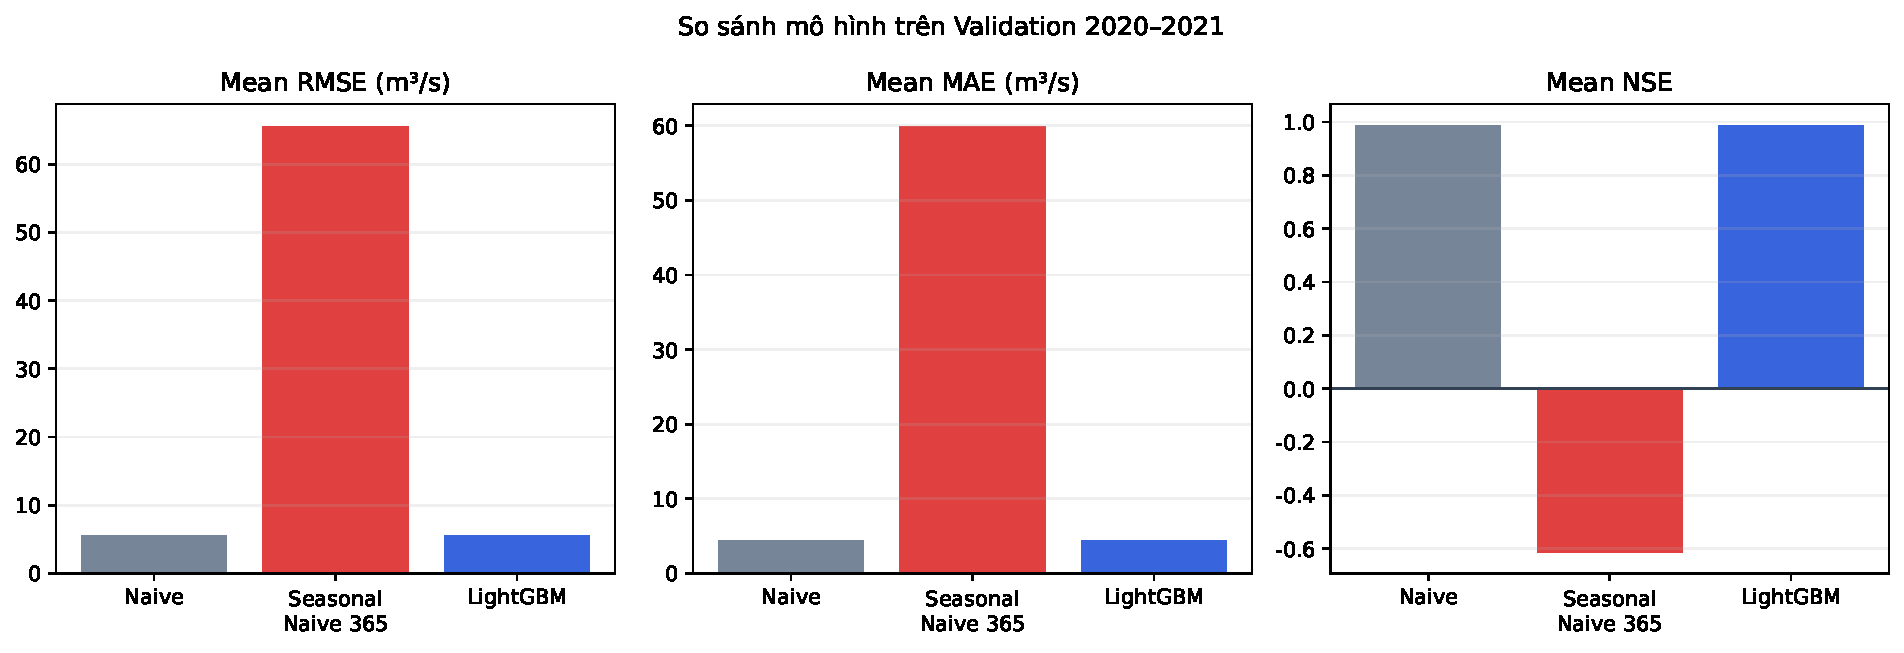
\includegraphics[width=0.86\linewidth]{validation_comparison.pdf}
\caption{So sánh RMSE, MAE và NSE trên Validation giữa ba mô hình.}
\label{fig:validation-comparison}
\end{figure}

Hình~\ref{fig:validation-comparison} cho thấy Seasonal Naive là mô hình kém nhất
trên Validation. Điều này phù hợp với phân tích ở câu hỏi 1: mùa vụ theo năm yếu và
mức nền thay đổi, nên việc lặp lại giá trị cùng ngày năm trước tạo sai số lớn.
LightGBM và Naive gần như trùng nhau; khoảng cách giữa hai mô hình nhỏ hơn nhiều so
với khoảng cách giữa chúng và Seasonal Naive.

\subsection{Kết quả Test tổng thể}

Bảng~\ref{tab:model-metrics} là kết quả chính trên Test 2022--2023. Naive có mean
RMSE 5,31, MAE 4,16 và NSE 0,881. LightGBM có mean RMSE 5,33, MAE 4,17 và NSE
0,881. Seasonal Naive có mean RMSE 60,48 và NSE $-13,333$. Như vậy, Naive là mô hình
tốt nhất theo mean RMSE, nhưng khoảng cách với LightGBM chỉ 0,02
m\textsuperscript{3}/s, tương đương khoảng 0,3\%. Về mặt thực hành, hai mô hình gần
như tương đương; về mặt thống kê, cần thêm dữ liệu để khẳng định mô hình nào thực
sự tốt hơn.

\begin{table}[H]
\centering
\small
\resizebox{\linewidth}{!}{\begin{tabular}{lrrrrr}
\toprule
Mô hình & mean RMSE & mean MAE & mean NSE & pooled RMSE & pooled NSE \\
\midrule
Naive persistence & 5{,}31 & 4{,}16 & 0{,}881 & 5{,}50 & 0{,}882 \\
Seasonal Naive 365 & 60{,}48 & 46{,}45 & -13{,}333 & 60{,}48 & -13{,}333 \\
LightGBM direct 7 (delta) & 5{,}33 & 4{,}17 & 0{,}881 & 5{,}52 & 0{,}881 \\
\bottomrule
\end{tabular}
}
\caption{Chỉ số dự báo trên Test 2022--2023. Mean là trung bình trên bảy horizon;
pooled là tính gộp toàn bộ 5.068 cặp dự báo.}
\label{tab:model-metrics}
\end{table}

Kết quả pooled cũng cho thấy cùng một bức tranh: Naive pooled RMSE 5,50, LightGBM
5,52, Seasonal 60,48. NSE pooled của Naive và LightGBM đều khoảng 0,881. Việc mean
và pooled gần nhau là do mỗi horizon có cùng số cặp dự báo; nếu số cặp giữa các
horizon khác nhau, hai cách tính có thể chênh lệch nhiều hơn.

Điểm đáng chú ý là Seasonal Naive rất kém trên Test, đặc biệt năm 2022. Nguyên nhân
là mức nền năm 2021 cao hơn nhiều so với 2022; khi lấy giá trị cùng ngày năm 2021
để dự báo 2022, mô hình lặp lại mức cao và tạo sai số lớn. Đây là ví dụ điển hình
cho việc một mô hình “có mùa vụ” vẫn có thể thất bại nếu mùa vụ không ổn định hoặc
mức nền thay đổi.

\subsection{Kết quả theo từng horizon}

Bảng~\ref{tab:metrics-horizon} trình bày chỉ số theo từng horizon. Với cả Naive và LightGBM, RMSE tăng gần như tuyến tính từ D+1
đến D+7: D+1 khoảng 2,79; D+7 khoảng 7,05--7,10. NSE giảm từ 0,970 ở D+1 xuống
0,802--0,804 ở D+7. Đây là quy luật hợp lý: dự báo càng xa càng khó, vì tính dai
dẳng giảm dần và các thay đổi mức nền có nhiều thời gian phát sinh hơn.

\begin{table}[H]
\centering
\small
\begin{tabular}{crrrrrr}
\toprule
Horizon & \multicolumn{3}{c}{Naive persistence} & \multicolumn{3}{c}{LightGBM direct 7} \\
\cmidrule(lr){2-4}\cmidrule(lr){5-7}
 & RMSE & MAE & NSE & RMSE & MAE & NSE \\
\midrule
D+1 & 2{,}79 & 2{,}23 & 0{,}970 & 2{,}79 & 2{,}23 & 0{,}970 \\
D+2 & 3{,}93 & 3{,}12 & 0{,}940 & 3{,}93 & 3{,}12 & 0{,}940 \\
D+3 & 4{,}87 & 3{,}85 & 0{,}907 & 4{,}87 & 3{,}85 & 0{,}907 \\
D+4 & 5{,}60 & 4{,}42 & 0{,}877 & 5{,}60 & 4{,}43 & 0{,}877 \\
D+5 & 6{,}23 & 4{,}91 & 0{,}848 & 6{,}25 & 4{,}93 & 0{,}846 \\
D+6 & 6{,}68 & 5{,}16 & 0{,}824 & 6{,}72 & 5{,}19 & 0{,}822 \\
D+7 & 7{,}05 & 5{,}40 & 0{,}804 & 7{,}10 & 5{,}45 & 0{,}802 \\
\bottomrule
\end{tabular}

\caption{Chỉ số theo horizon trên Test 2022--2023.}
\label{tab:metrics-horizon}
\end{table}

Ở D+1, D+2 và D+3, hai mô hình gần như trùng nhau đến hai chữ số thập phân. Từ D+5
trở đi, LightGBM bắt đầu kém hơn một chút: D+7 có RMSE 7,10 so với 7,05 của Naive,
MAE 5,45 so với 5,40, NSE 0,802 so với 0,804. Mức chênh lệch này nhỏ nhưng có hệ
thống, cho thấy các đặc trưng bổ sung chưa giúp ích cho horizon dài. Một phần nguyên
nhân là mô hình delta phải học phần thay đổi nhỏ giữa hai mức lưu lượng, trong khi
phần thay đổi này chịu ảnh hưởng của nhiều yếu tố không có trong dữ liệu.

\subsection{Kết quả theo năm}

Bảng~\ref{tab:metrics-year} và Hình~\ref{fig:error-year} cho thấy sai số thay đổi
theo năm. Năm 2022 có RMSE khoảng 5,26--5,27 cho Naive và LightGBM, nhưng NSE chỉ
khoảng 0,67. Năm 2023 có RMSE cao hơn một chút (5,36--5,38) nhưng NSE cao hơn
(0,885--0,886). NSE phụ thuộc vào phương sai của mục tiêu trong từng năm: nếu lưu
lượng ít biến động, một RMSE nhỏ vẫn có thể tạo NSE thấp. Vì vậy cần đọc RMSE và
NSE cùng nhau, không nên chỉ dựa vào một chỉ số.

\begin{table}[H]
\centering
\small
\begin{tabular}{lrrrr}
\toprule
Mô hình & Năm & RMSE & MAE & NSE \\
\midrule
Naive persistence & 2022 & 5{,}26 & 4{,}12 & 0{,}670 \\
Naive persistence & 2023 & 5{,}36 & 4{,}19 & 0{,}886 \\
Seasonal Naive 365 & 2022 & 82{,}43 & 74{,}10 & -74{,}054 \\
Seasonal Naive 365 & 2023 & 22{,}85 & 18{,}79 & -0{,}949 \\
LightGBM direct 7 (delta) & 2022 & 5{,}27 & 4{,}12 & 0{,}668 \\
LightGBM direct 7 (delta) & 2023 & 5{,}38 & 4{,}22 & 0{,}885 \\
\bottomrule
\end{tabular}

\caption{Chỉ số theo năm trên Test.}
\label{tab:metrics-year}
\end{table}

\begin{figure}[H]
\centering
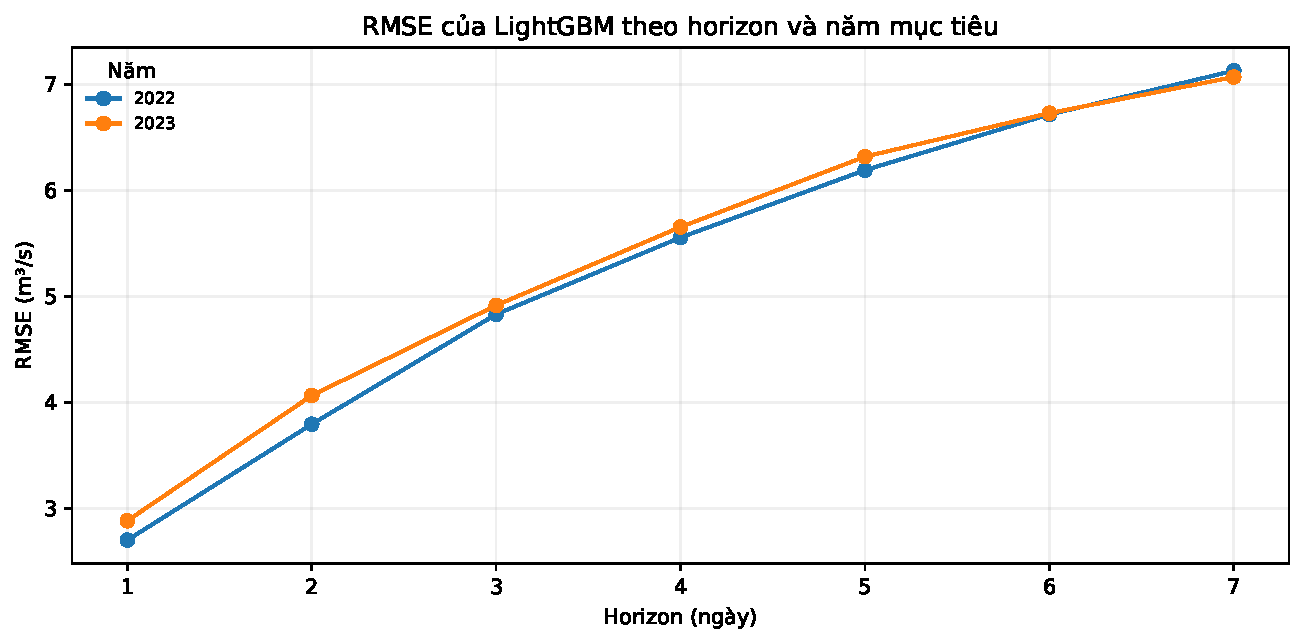
\includegraphics[width=0.82\linewidth]{error_by_year.pdf}
\caption{RMSE của LightGBM theo horizon và năm mục tiêu (2022, 2023).}
\label{fig:error-year}
\end{figure}

Seasonal Naive có RMSE 82,43 vào năm 2022 và 22,85 vào năm 2023. NSE năm 2022 là
$-74,054$, phản ánh việc mô hình lặp lại mức lưu lượng cao của năm 2021 trong khi
thực tế năm 2022 thấp hơn nhiều. Đây là minh chứng mạnh nhất cho việc không nên dùng
Seasonal Naive cho chuỗi có mức nền thay đổi.

\subsection{Mức độ quan trọng của đặc trưng}

Bảng~\ref{tab:feature-importance} và Hình~\ref{fig:feature-importance} tổng hợp
mean gain của các đặc trưng qua bảy mô hình. Đứng đầu là
\texttt{target\_doy\_sin\_h7}, tiếp theo là \texttt{target\_doy\_sin\_h6},
\texttt{lag\_30}, \texttt{target\_doy\_sin\_h5} và \texttt{roll\_std\_30}. Việc các
đặc trưng lịch của ngày mục tiêu xuất hiện ở nhóm đầu cho thấy mô hình sử dụng vị
trí mùa để điều chỉnh dự báo, dù mùa vụ yếu. Các lag dài (28, 30 ngày) và độ lệch
chuẩn rolling 30 ngày cũng quan trọng, phản ánh mức nền và độ bất định gần đây.

\begin{table}[H]
\centering
\footnotesize
\setlength{\tabcolsep}{3.2pt}
\begin{tabular}{rlrr}
\toprule
Hạng & Feature & Mean gain & Tỷ trọng (\%) \\
\midrule
1 & \texttt{target\_doy\_sin\_h7} & 16.171{,}46 & 16{,}50 \\
2 & \texttt{target\_doy\_sin\_h6} & 12.170{,}66 & 12{,}42 \\
3 & \texttt{lag\_30} & 11.432{,}03 & 11{,}67 \\
4 & \texttt{target\_doy\_sin\_h5} & 8.869{,}39 & 9{,}05 \\
5 & \texttt{roll\_std\_30} & 7.023{,}35 & 7{,}17 \\
6 & \texttt{target\_month\_cos\_h7} & 4.714{,}40 & 4{,}81 \\
7 & \texttt{lag\_28} & 4.212{,}61 & 4{,}30 \\
8 & \texttt{target\_doy\_cos\_h5} & 3.904{,}04 & 3{,}98 \\
9 & \texttt{roll\_std\_14} & 3.583{,}02 & 3{,}66 \\
10 & \texttt{target\_doy\_cos\_h7} & 2.978{,}14 & 3{,}04 \\
11 & \texttt{target\_doy\_h7} & 2.299{,}89 & 2{,}35 \\
12 & \texttt{origin\_doy\_sin} & 1.982{,}94 & 2{,}02 \\
13 & \texttt{target\_month\_cos\_h6} & 1.852{,}88 & 1{,}89 \\
14 & \texttt{target\_doy\_cos\_h4} & 1.800{,}94 & 1{,}84 \\
15 & \texttt{target\_month\_cos\_h5} & 1.151{,}80 & 1{,}18 \\
\bottomrule
\end{tabular}

\caption{15 đặc trưng có mean gain cao nhất, tổng hợp qua bảy mô hình horizon.}
\label{tab:feature-importance}
\end{table}

\begin{figure}[H]
\centering
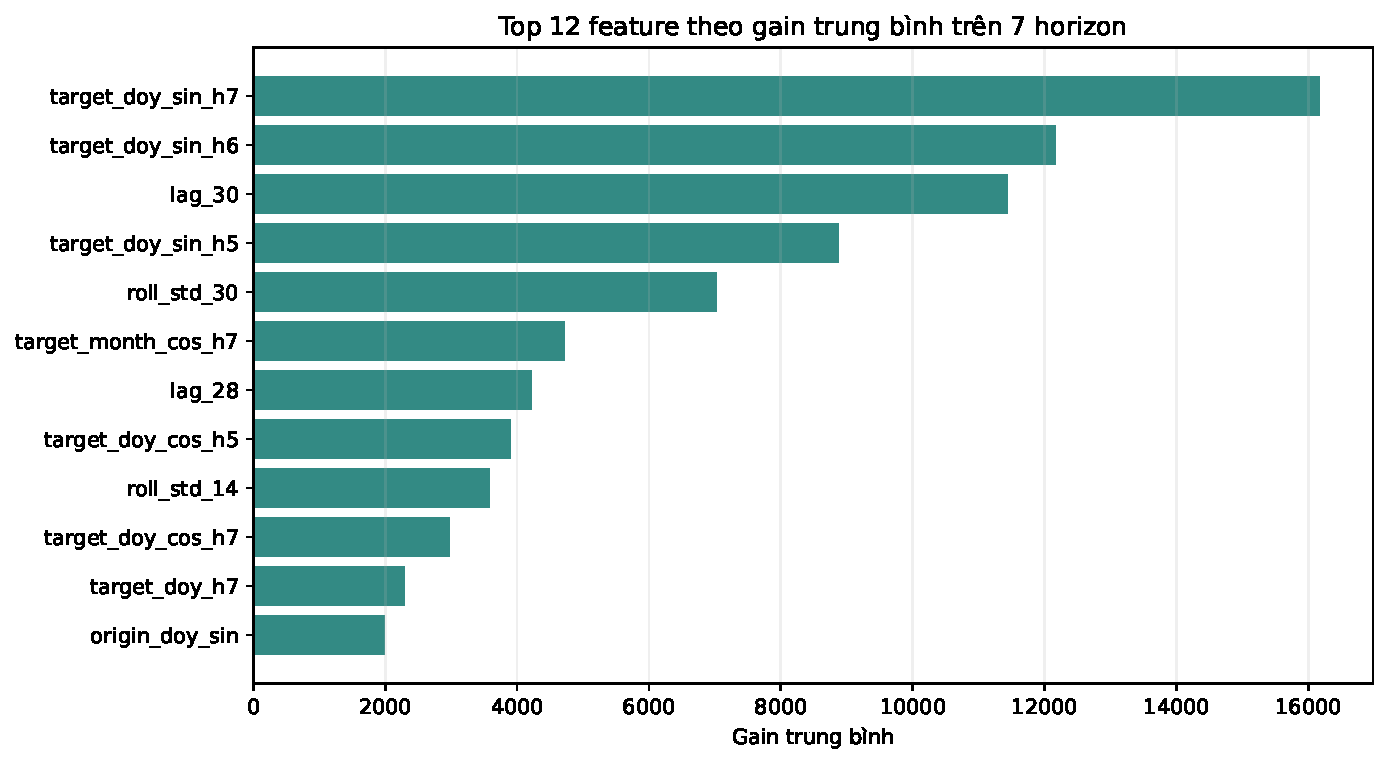
\includegraphics[width=0.88\linewidth]{feature_importance.pdf}
\caption{Mean gain của các đặc trưng LightGBM.}
\label{fig:feature-importance}
\end{figure}

Cần thận trọng khi diễn giải gain: đây là thước đo mức đóng góp của đặc trưng trong
các cây đã học, không phải quan hệ nhân quả. Một đặc trưng có gain cao có thể chỉ
đang giúp mô hình chia tách các giai đoạn mức nền, chứ không chứng minh rằng nó tạo
ra lưu lượng. Ngoài ra, gain được tổng hợp qua các horizon có thang đo khác nhau;
so sánh giữa các horizon nên được thực hiện riêng, không chỉ dựa vào bảng tổng hợp.

\subsection{Chẩn đoán phần dư và ví dụ dự báo}

Hình~\ref{fig:residual-distribution} và Hình~\ref{fig:forecast-scatter} cho thấy
phần dư của LightGBM phân bố quanh 0 nhưng độ rộng tăng theo horizon. Ở D+1, phần
lớn sai số nằm trong khoảng $\pm 4$ m\textsuperscript{3}/s; ở D+7, khoảng sai số mở
rộng lên khoảng $\pm 12$ m\textsuperscript{3}/s. Bias trung bình của LightGBM là
0,27 m\textsuperscript{3}/s, trong khi Naive là 0,07; bias nhỏ so với RMSE, nhưng
cho thấy mô hình có xu hướng dự báo cao hơn thực tế một chút.

\begin{figure}[H]
\centering
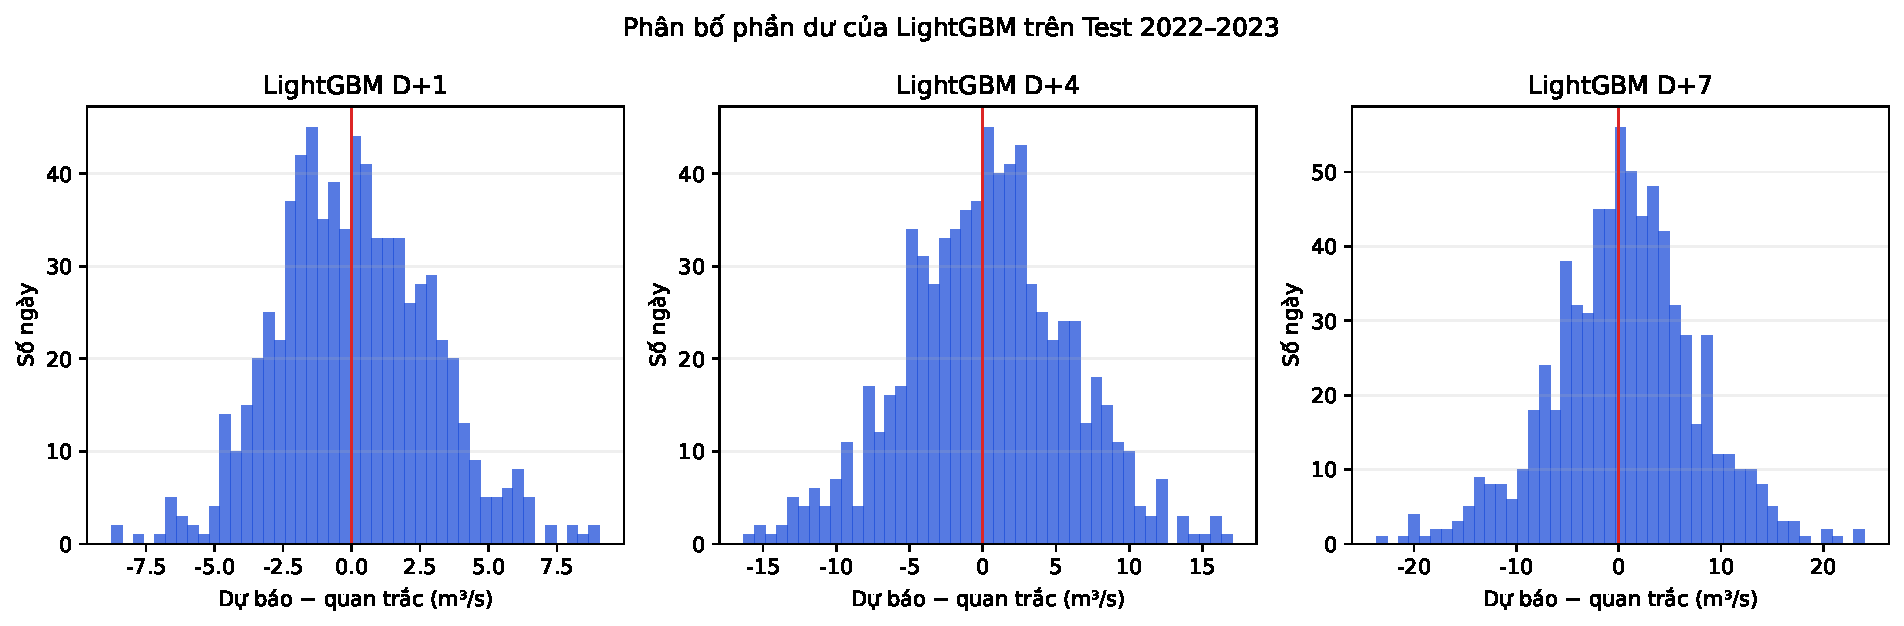
\includegraphics[width=0.84\linewidth]{residual_distribution.pdf}
\caption{Phân bố phần dư của LightGBM trên Test.}
\label{fig:residual-distribution}
\end{figure}

\begin{figure}[H]
\centering
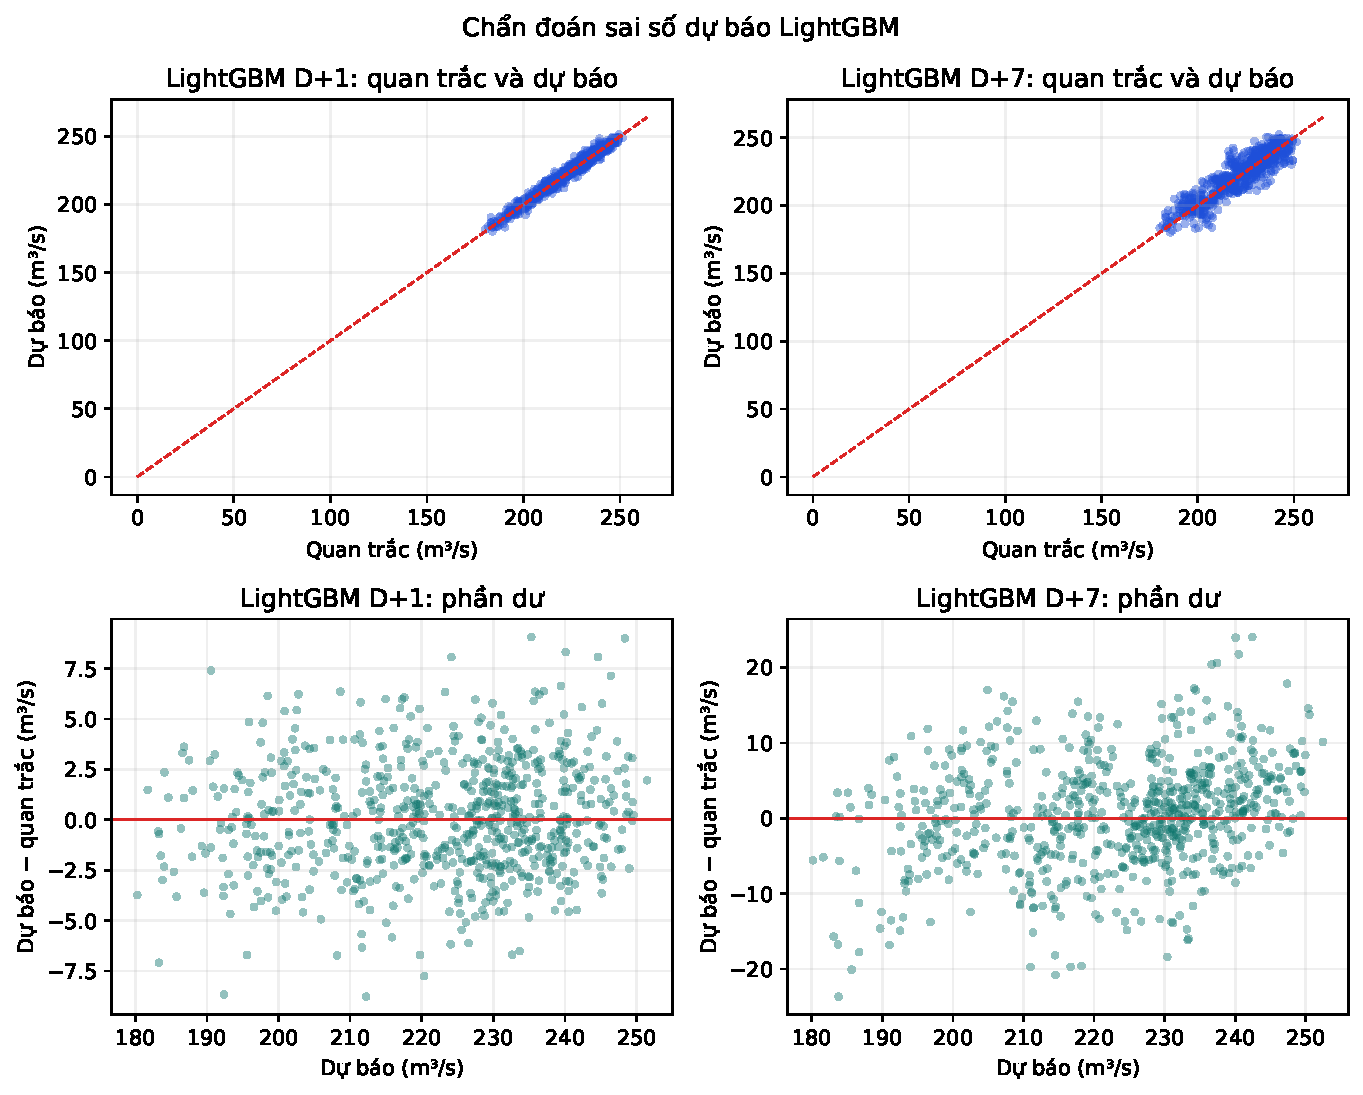
\includegraphics[width=0.84\linewidth]{forecast_scatter.pdf}
\caption{Quan trắc và dự báo của LightGBM ở D+1 và D+7, kèm phần dư.}
\label{fig:forecast-scatter}
\end{figure}

Hình~\ref{fig:forecast-hydrograph} minh họa dự báo rolling-origin trên toàn bộ Test.
Cả Naive và LightGBM bám sát chuỗi quan trắc; Seasonal Naive tạo các đoạn nhảy lớn
khi mức nền giữa các năm thay đổi. Đây là hình ảnh trực quan của kết quả trong
Bảng~\ref{tab:model-metrics}: mô hình đơn giản nhất lại là mô hình khó bị đánh bại
trong chuỗi này.

\begin{figure}[H]
\centering
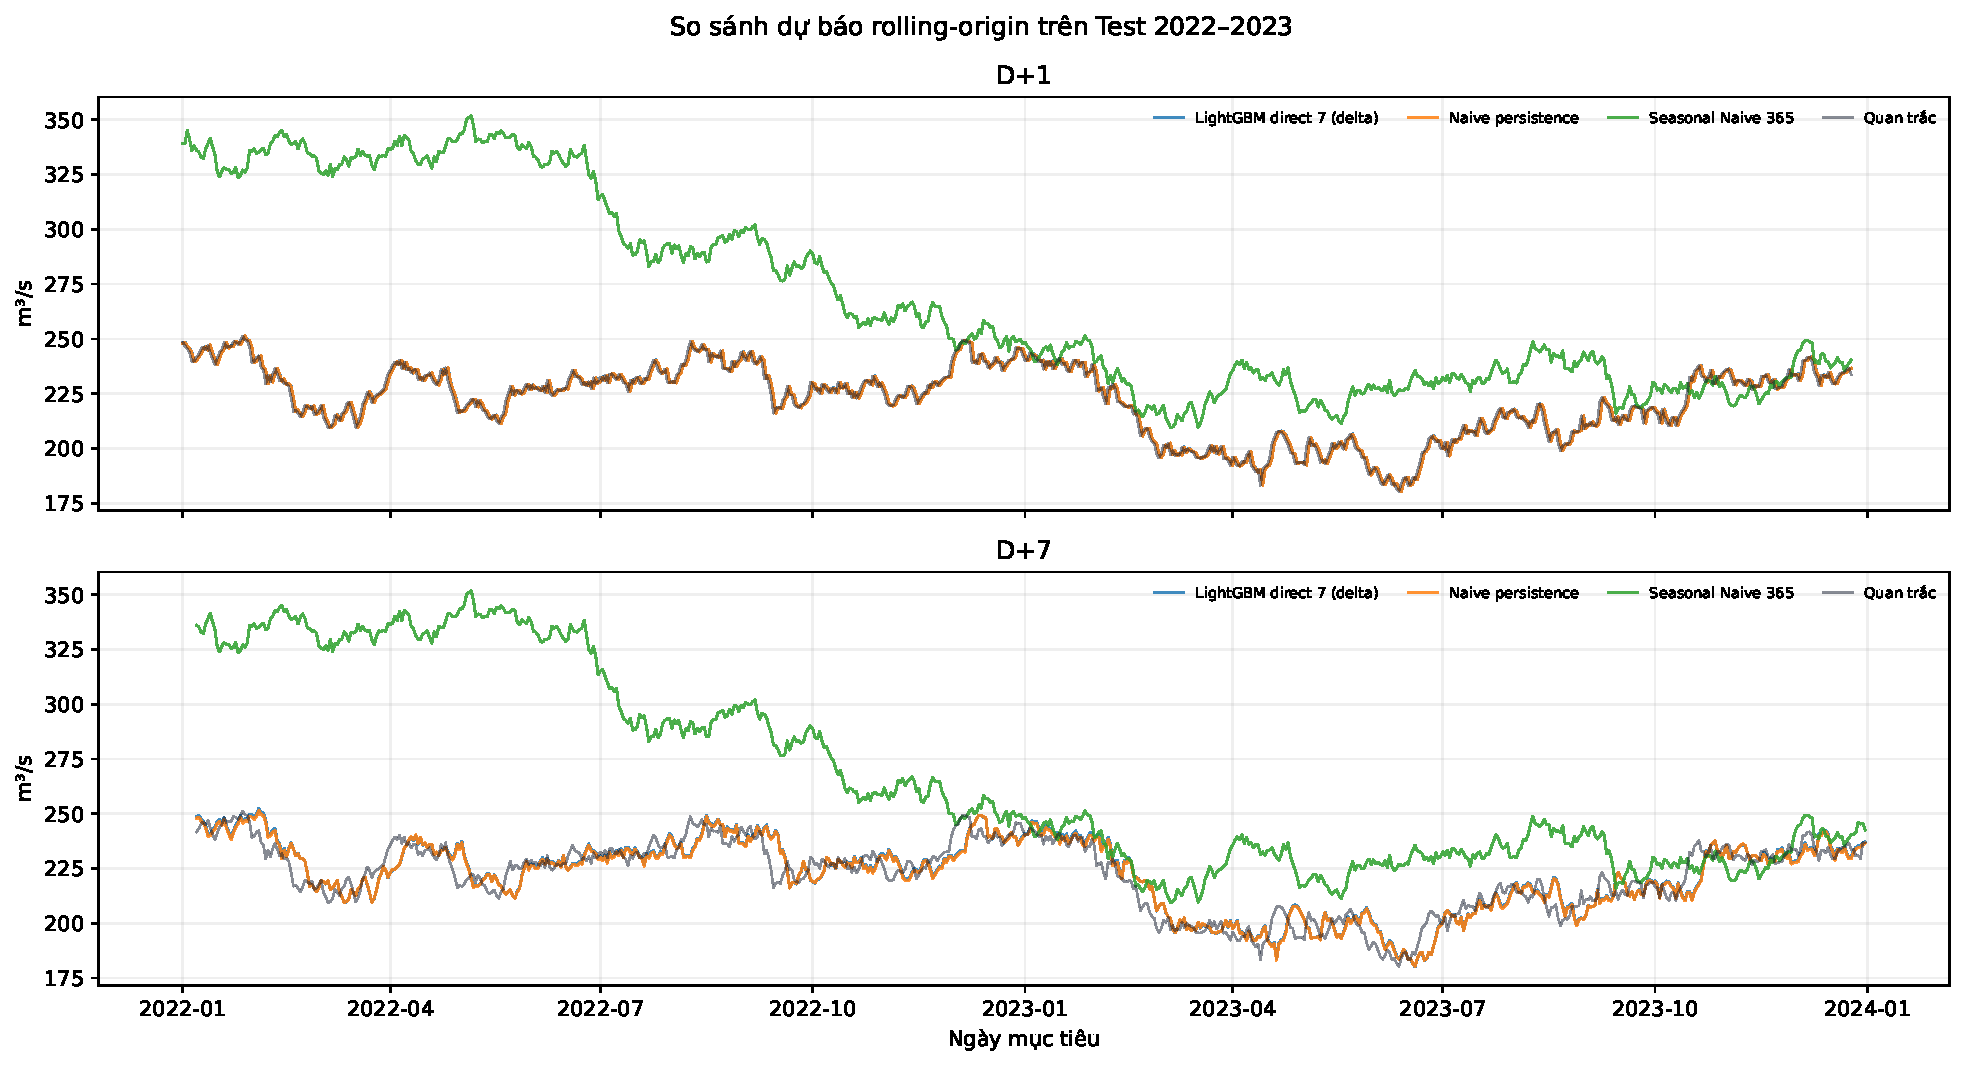
\includegraphics[width=0.96\linewidth]{forecast_hydrograph.pdf}
\caption{Dự báo rolling-origin ở D+1 và D+7 trên Test 2022--2023.}
\label{fig:forecast-hydrograph}
\end{figure}

Một hạn chế quan trọng là Test 2022--2023 không có ngày nào vượt Q95. Vì vậy báo cáo
\emph{không thể} đánh giá khả năng dự báo cực trị của mô hình. Các chỉ số tốt trên
Test chủ yếu phản ánh khả năng bám mức nền và biến động thông thường, không phản ánh
khả năng cảnh báo lũ. Nếu muốn đánh giá cực trị, cần một tập Test có ít nhất một số
đợt vượt ngưỡng, hoặc dùng thiết kế đánh giá riêng cho các đợt cực trị.

\subsection{Trả lời câu hỏi 3}

Các kết quả chính:

\begin{itemize}[leftmargin=1.4em]
  \item LightGBM direct 7 đạt mean RMSE 5,33 và NSE 0,881 trên Test, gần tương
  đương Naive (5,31 và 0,881) và tốt hơn rất nhiều so với Seasonal Naive 365
  (60,48 và $-13,333$).
  \item Khoảng cách LightGBM--Naive chỉ khoảng 0,02 m\textsuperscript{3}/s
  (0,3\%); không có bằng chứng thuyết phục rằng mô hình học máy vượt trội.
  \item Sai số tăng theo horizon: D+1 có RMSE khoảng 2,79 và NSE 0,970; D+7 có
  RMSE khoảng 7,10 và NSE 0,802.
  \item Năm 2022 khó hơn 2023 theo NSE; Seasonal Naive thất bại nặng vào 2022 do
  mức nền thay đổi.
  \item Test không có ngày vượt Q95, nên không thể kết luận về khả năng dự báo
  cực trị từ kết quả này.
\end{itemize}

Kết luận thực hành là: trong chuỗi có tính dai dẳng cao và mùa vụ yếu, một baseline
đơn giản như Naive là đối thủ mạnh. LightGBM có thể dùng để thử nghiệm các đặc
trưng bổ sung, nhưng cần đánh giá cẩn thận và không nên mặc định rằng mô hình phức
tạp hơn sẽ tốt hơn.
